\chapter{Group~II: Ordering along a Line}\label{chapter:LinearOrder}
\section{Overview}
In the first two axioms, Hilbert asserts that two distinct points uniquely determine a line. Similarly, in the fourth and fifth axioms, he asserts that three non-collinear points uniquely determine a plane. We can then ask about the converse: firstly, is every line determined by at least two points; and secondly, is every plane determined by at least three non-collinear points? Both questions were answered axiomatically in the first edition:

\begin{quote}
  \begin{enumerate}
  \item[I,7]. Upon every straight line there exist at least two points, in every plane at least three points not lying in the same straight line.
  \end{enumerate}
\end{quote}

By the tenth edition, the first property had migrated to the first part of Axiom~I,3 (see Figure \ref{fig:GroupI}). But now it is rendered more ambiguously. It could be the very weak claim that there exists a line and two points on it, or the stronger claim that \emph{every} line has two points on it. We assumed the latter, since on the weaker interpretation, we could formalise a model of the first group of axioms following the technique in \ref{sec:GroupIModels}, and show in this model that there is a line with \emph{no} incident points. We assume Hilbert did not intend this. 

The second property in Axiom I,7 was replaced by a weak clause in the fourth axiom, saying that a plane contains at least one point. The remaining axioms are then sufficient to prove the following:

\begin{theorem}\label{theorem:PlaneHasThreePoints}
Every plane $\alpha$ contains at least three non-collinear points.
\end{theorem}
\begin{proof}
By $I,4$ and $I,8$, we can take a point $A$ on $\alpha$ and a point $B$ not on $\alpha$. We connect these two points by a line $a$. By $I,3$, we can take a third point $C$ off the line $a$. The three points $A$,$B$ and $C$ must determine a plane $\beta$ by $I,4$. 

Since the planes $\alpha$ and $\beta$ intersect at the point $A$, we can choose another intersection point $D$ by $I,7$, and by $I,8$, we can find a fifth point $E$ off the plane $\beta$. Now $A$,$B$ ad $E$ must be non-collinear, and so they determine a plane $\gamma$. If this plane is $\alpha$, then $A$, $B$ and $E$ are our three points and we are done. Otherwise, we have two distinct planes intersecting at $A$ and so we can take another intersection point $F$ by $I,7$. This gives us three non-collinear points in $\alpha$, namely $A$, $D$ and $F$.
\end{proof}

The formalised version is given in Figure~\ref{fig:PlaneHasThreePoints}\footnote{The formalised axioms are given in Appendix~\ref{app:GroupIFormalisation}}, where there is more detailed cross-referencing of the axioms. We see that Axiom I,6 is employed to locate points on planes, and we see how the proof that $A$, $D$ and $F$ is non-collinear becomes two subproofs which draw on the other incidence axioms.

\begin{figure}
  \begin{enumerate}
  \item[I,1] For every two points $A$, $B$ there exists a line $a$ that contains each of the points $A$, $B$.
  \item[I,2] For every two points $A$, $B$ there exits [sic] no more than one line that contains each of the points $A$, $B$.
  \item[I,3] There exist at least two points on a line. There exist at least three points that do not lie on a line.
  \item[I,4] For any three points $A$, $B$, $C$ that do not lie on the same line there exits [sic] a plane $\alpha$ that contains each of the points $A$, $B$, $C$. For every plane there exists a point which it contains.
  \item[I,5] For any three points $A$, $B$, $C$ that do not lie on one and the same line there exists no more than one plane that contains each of the three points $A$, $B$, $C$.
  \item[I,6] If two points $A$, $B$ of a line $a$ lie in a plane $\alpha$ then every point of $a$ lies in the plane $\alpha$.
  \item[I,7] If two planes $\alpha$, $\beta$ have a point $A$ in common then they have at least one more point $B$ in common.
  \item[I,8] There exist at least four points which do not lie in a plane.
  \end{enumerate}
  \caption{Group I axioms}
  \label{fig:GroupI}
\end{figure}

\begin{figure}
\small
\begin{align*}
&\texttt{theorem }\forall\alpha.\,\exists A\,B\,C.\,\onplane{A}{\alpha} \wedge \onplane{B}{\alpha} \wedge  \onplane{C}{\alpha}\\
&\qquad\wedge  \Triangle{a}{A}{B}{C}\\
&\texttt{fix } \alpha\\
&\texttt{consider } A \texttt{ at 0 such that } \onplane{A}{\alpha} \texttt{ by g14b}\\
&\texttt{consider } B \texttt{ at 1 such that } \neg \onplane{B}{\alpha} \texttt{ by g18}\\
&\texttt{have } A \neq B \texttt{ at 2 from 0,1}\\
&\texttt{so consider } a \texttt{ at 3 such that } \online{A}{a} \wedge  \online{B}{a} \texttt{ by g11}\\
&\texttt{consider } C \texttt{ at 4 such that } \neg \online{C}{a} \texttt{ by g13b}\\
&\texttt{have } \Triangle{b}{A}{B}{C}\\
&\quad\texttt{otherwise consider } b \texttt{ at 5 such that }\online{A}{b}\wedge \online{B}{b}\wedge \online{C}{b}\\
&\quad\texttt{hence } a = b \texttt{ from 2,3 by g12}\\
&\quad\texttt{qed from 4,5}\\
&\texttt{so consider } \beta \texttt{ at 5 such that }\\
&\quad\onplane{A}{\beta}\wedge \onplane{B}{\beta}\wedge \onplane{C}{\beta} \texttt{ by g14a}\\
&\texttt{consider } D \texttt{ at 6 such that } \onplane{D}{\alpha}\wedge \onplane{D}{\beta}\wedge A\neq D \\
&\qquad\texttt{ from 0,1,5 by g17}\\
&\texttt{consider } E \texttt{ at 7 such that } \neg \onplane{E}{\beta} \texttt{ by g18}\\
&\texttt{have } \Triangle{b}{A}{B}{E} \texttt{ at 8}\\
&\quad\texttt{otherwise consider } b \texttt{ at 9 such that }\online{A}{b}\wedge \online{B}{b}\wedge  \online{E}{b}\\
&\quad\texttt{hence }\onplane{E}{\beta} \texttt{ from 2,5 by g16}\\
&\quad\texttt{qed from 7}\\
&\texttt{so consider } \gamma \texttt{ at 9 such that}\\
&\quad\onplane{A}{\gamma}\wedge \onplane{B}{\gamma}\wedge \onplane{E}{\gamma}\texttt{ by g14a}\\
&\texttt{assume } \alpha\neq\gamma \texttt{ from 8,9}\\
&\texttt{so consider } F \texttt{ at 10 such that }\onplane{F}{\alpha}\wedge \onplane{F}{\gamma}\wedge A \neq F \\
&\quad\texttt{ from 0,9 by g17}\\
&\texttt{have }\Triangle{b}{A}{D}{F}\\
&\quad\texttt{otherwise consider } b \texttt{ at 11 such that }\\
&\quad\quad\online{A}{b}\wedge \online{D}{b}\wedge \online{F}{b}\\
&\quad\texttt{hence }\onplane{D}{\gamma}\texttt{ at 12 from 0,9,10 by g16}\\
&\quad\texttt{have }\Triangle{c}{A}{B}{D}\\
&\quad\quad\texttt{otherwise consider } c \texttt{ at 13 such that }\\
&\quad\quad\quad\online{A}{c}\wedge \online{B}{c}\wedge \online{D}{c}\\
&\quad\quad\texttt{hence }\onplane{B}{\alpha}\texttt{ from 0,6 by g16}\\
&\quad\quad\texttt{qed from 1}\\
&\quad\texttt{hence }\beta=\gamma \texttt{ from 5,6,9,12 by g15}\\
&\quad\texttt{qed from 7,9}\\
&\texttt{qed from 0,6,10}
\end{align*}
\caption{Formalised proof of Theorem \ref{theorem:PlaneHasThreePoints}}
\label{fig:PlaneHasThreePoints}
\end{figure}

\section{Models}
We formalised the axioms as a higher-order two-place predicate \texttt{group1} over relations $\text{on\_line}$ and $\text{on\_plane}$. The primitive domains of points, lines and planes is then given in the types of these arguments.

Since types must be inhabited in simple type theory, this puts a stronger constraint on the axioms than Hilbert perhaps intended. However, if we consider a single type for points, lines and planes, we can relativise every axiom against the predicate sets \texttt{is\_point}, \texttt{is\_line} and \texttt{is\_plane}. For instance, the first axiom becomes:
\begin{align*}
\forall A\, B.\, \texttt{is\_point} A &\wedge  \texttt{is\_point} B \implies A \neq B\\
&\implies \exists a.\, \texttt{is\_line}\,a \wedge \online{A}{a} \wedge \online{B}{a}
\end{align*}

These axioms no longer make the existential assumptions implied by simple type theory. Instead, we must formally prove $\exists A.\,\texttt{is\_point}\,A$, $\exists a.\,\texttt{is\_line}\,a$ and $\exists \alpha.\,\texttt{is\_plane}\,\alpha$. To do this, we use axioms \texttt{g11}, \texttt{g13b}, \texttt{g14} and \texttt{g18} as follows: by Axiom \texttt{g13b}, we have a non-collinear triple of points. We might assume that these give us the lines of a triangle. However, the points are not necessarily distinct: they might be non-collinear simply because there do not exist any lines!

Thus, we must now obtain a plane from axiom \texttt{g14}, and then use \texttt{g18} to give us a second point not in this plane. This point we know to be distinct from the three others, and thus, we have a line from \texttt{g11}.

Because none of Hilbert's theorems require polymorphic types, it is possible to use the \texttt{group1} predicate as a condition on all theorems without extending the basic axioms of higher-order logic. Moreover, the predicate allows us to exhibit various models of the axioms, any of which guarantee the axioms' consistency. However, this makes it more difficult to define new objects in the theory, since every new defined term must carry two arguments for the incidence properties. Since Hilbert creates fairly elaborate towers of definitions just to state his later axioms, we decided to extend higher-order logic axiomatically:

\begin{displaymath}
\vdash \texttt{group1}\,\texttt{on\_line}\,\texttt{on\_plane}.
\end{displaymath}

\subsection{The Minimal Model}\label{sec:GroupIModels}
Hilbert's first group of axioms can be realised in the four vertices, six lines, and four planes of a tetrahedron. In such a finite interpretation, we can translate the first-order axioms into propositional axioms and verify them with a tautology checker.

To capture this idea formally, we carved out two finite types, one with exactly four constructors used as interpretations of the four points and the four planes in our model, and the other with exactly six constructors used as the interpretations of the six lines.

\begin{align*}
\texttt{ps}   &= \texttt{p1} \vert \texttt{p2} \vert\texttt{p3} \vert\texttt{p4}\\
\texttt{lines}&= \texttt{l1} \vert \texttt{l2} \vert\texttt{l3} \vert\texttt{l4} \vert\texttt{l5} \vert\texttt{l6}\\
\end{align*}

The type definitions are used to automatically derive an abstract type and derive two theorems, an induction theorem and a recursion theorem. For the type \texttt{ps}, for instance, we are given

\begin{align*}
&\forall P. P\,\texttt{p1}\,\wedge\,P\,\texttt{p2}\,\wedge\,P\,\texttt{p3}\,\wedge\,P\,\texttt{p4}\implies\forall p. P\,p\\
&\forall p1\,p2\,p3\,p4. \exists f. f\,\texttt{p1} = p1\,\wedge\,f\,\texttt{p2} = p2\,\wedge\,f\,\texttt{p3} = p3\,\wedge\,f\,\texttt{p4} = p4.
\end{align*}

The first (induction) theorem can be promoted to an equivalence, and then used to rewrite all universally quantified statements as finite conjunctions. Similarly, its rewrite using the infinite DeMorgan rule, $(\forall x. P\,x) \iff \neg\exists x. \neg (P\,x)$ can be used to rewrite all existentially quantified statements as finite disjunctions.

Next, by instantiating the universally quantified variables in the second (recursion) theorem with the first four natural numbers respectively, we can prove that \texttt{p1}, \texttt{p2}, \texttt{p3} and \texttt{p4} are mutually distinct. From this, every valid first-order formula over the types \texttt{ps} and \texttt{lines} can be rewritten to a mere tautology and then quickly verified.

To check our model, we first inductively define the incidence predicates on\_line and on\_plane over the types \texttt{ps} and \texttt{lines}, as shown in Figure~\ref{fig:SmallestModel}. We were then able to formalise the following theorem in HOL~Light 
\begin{displaymath}
\vdash \text{Group1}\,\text{online}\,\text{onplane}.
\end{displaymath}

\begin{figure}
\begin{minipage}[c]{5cm}
\begin{align*}
& \online{\texttt{p1}}\texttt{l1}\wedge \online{\texttt{p2}}\texttt{l1}\\
\wedge & \online{\texttt{p1}}\texttt{l2}\wedge \online{\texttt{p3}}\texttt{l2}\\
\wedge & \online{\texttt{p2}}\texttt{l3}\wedge \online{\texttt{p3}}\texttt{l3}\\
\wedge & \online{\texttt{p1}}\texttt{l4}\wedge \online{\texttt{p4}}\texttt{l4}\\
\wedge & \online{\texttt{p2}}\texttt{l5}\wedge \online{\texttt{p4}}\texttt{l5}\\
\wedge & \online{\texttt{p3}}\texttt{l6}\wedge \online{\texttt{p4}}\texttt{l6}\\
\\
& \onplane{\texttt{p1}}{\texttt{p1}}\wedge \onplane{\texttt{p2}}{\texttt{p1}}\wedge \onplane{\texttt{p3}}{\texttt{p1}}\\
\wedge & \onplane{\texttt{p1}}{\texttt{p2}}\wedge \onplane{\texttt{p2}}{\texttt{p2}}\wedge \onplane{\texttt{p4}}{\texttt{p2}}\\
\wedge & \onplane{\texttt{p1}}{\texttt{p3}}\wedge \onplane{\texttt{p3}}{\texttt{p3}}\wedge \onplane{\texttt{p4}}{\texttt{p3}}\\
\wedge & \onplane{\texttt{p2}}{\texttt{p4}}\wedge \onplane{\texttt{p3}}{\texttt{p4}}\wedge \onplane{\texttt{p4}}{\texttt{p1}}
\end{align*}\end{minipage}%\scalebox{0.3}{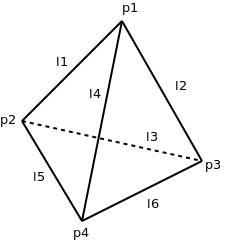
\includegraphics{tetra}}
\caption{Smallest model}\label{fig:SmallestModel}
\end{figure}

After unfolding the definitions of $\text{on\_line}$ and $\text{on\_plane}$, it turns out that the theorem can be proven by equational reasoning alone. We replace the universals and existentials with conjunctions and disjunctions respectively. After simplifying, the remaining goals require us to show that points, lines or planes are distinct, which is dealt with by the recursion theorem.

The same method allows us to formally deal with the case of a weakened axiom \texttt{g13a}. Here we define a seven element finite set for the lines, and use the same inductive definitions for \texttt{on\_line} and \texttt{on\_plane}, leaving the seventh line ``dangling'' without any incident points. Again, by rewriting the axioms propositionally and simplifying, we can show that this is a (presumably inappropriate) model for the weakened axioms.

To show that the tetrahedron model is minimal, we proved that there exist four points, six lines and four planes satisfying the conditions we gave to inductively define \texttt{on\_line} and \texttt{on\_plane} in the model. We know from Theorem~\ref{theorem:PlaneHasThreePoints} that there are three distinct points on a plane. From axiom \texttt{g18}, there is a fourth point not on this plane. The remaining axioms are then sufficient to connect each pair of points by a unique line.

\section{Group~2 Overview}
The next group of axioms concern \emph{order} and \emph{orientation} in terms of a primitive three-place predicate $\text{between}$. In our formalisation, we use this predicate in terms such as $\text{between}\,A\,B\,C$, which we interpret as saying that the point $B$ lies between the points $A$ and $C$. The axioms are given in Figure \ref{fig:GroupII} and the formalisation in Appendix \ref{app:GroupIIFormalisation}.

\begin{figure}
  \begin{enumerate}
  \item[II,1] If a point $B$ lies between a point $A$ and a point $C$ then the points $A,B,C$ are three distinct points of a line, and $B$ then also lies between $C$ and $A$.
  \item[II,2] For two points $A$ and $C$, there always exists at least one point $B$ on the line $AC$ such that $C$ lies between $A$ and $B$.
  \item[II,3] Of any three points on a line there exists no more than one that lies between the other two.
  \item[II,4] Let $A$, $B$, $C$ be three points that do not lie on a line and let $a$ be a line in the plane $ABC$ which does not meet any of the points $A$, $B$, $C$. If the line $a$ passes through a point of the segment $AB$, it also passes through a point of the segment $AC$, or through a point of the segment $BC$.
  \end{enumerate}
  \caption{Group II axioms}
  \label{fig:GroupII}
\end{figure}

These axioms have been heavily revised since the first edition as various redundancies were discovered. Originally, Axiom~II,2 had an additional clause asserting that we can always find a point between two others. This turned out to be derivable, and we give its proof and formalisation in \S\ref{sec:Theorem3}. The quantification in Axiom~II,3 was stronger, claiming that, given three points, there is \emph{exactly} one that lies between the other two. By the tenth edition, the existence of the point was derived as Theorem~4 in a proof attributed to Wald~\cite{FoundationsOfGeometry}. Finally, a ``transitivity'' axiom was removed to become Theorem~5, the proof due to Moore~\cite{MooreProof}.

\begin{quote}
  \begin{enumerate}
  \item[I,4]. Any four points $A, B, C, D$ of a straight line can always be so arranged that $B$ shall lie between $A$ and $C$ and also between $A$ and $D$, and, furthermore, that $C$ shall lie between $A$ and $D$ and also between $B$ and $D$.
  \end{enumerate}
\end{quote}

After revising, the Group~II axioms consist of constraints on the between relation, an axiom to extend a line segment in a given direction, and finally a planar axiom of order. This last axiom, depicted in Figure~\ref{fig:PaschDiagram}, was identified by Pasch as a crucial missing postulate from Euclid's Elements~\cite{Heath?}. It appears the most complex of the axioms so far, being a planar axiom with numerous preconditions and a disjunctive conclusion, and it is used heavily in the proofs of Theorem~4 and Theorem~5. Each of these proofs starts with a linear assumption, builds a planar diagram, and then uses Pasch to produce a linear conclusion.

\begin{figure}
% \begin{pspicture}(-2,0)(5,3.5)
% \psset{xunit=0.75cm}
% \psset{yunit=0.5cm}
% \put(1.3,0.2){\parbox{5cm}{$A$}}
% \put(6,0.2){\parbox{5cm}{$B$}}
% \put(5.2,2.6){\parbox{5cm}{$C$}}
% \put(2.1,2.0){\parbox{5cm}{$a$}}
% \put(4.8,1.1){\parbox{5cm}{$a$}}
% \put(5.7,1.7){\parbox{5cm}{$F$}}
% \put(3.2,1.7){\parbox{5cm}{$F$}}
% \put(2.8,0.0){\parbox{5cm}{$D$}}
% \put(4.7,0.0){\parbox{5cm}{$D$}}
% \put(6.8,2.0){\parbox{5cm}{$E$}}
% \put(1.2,3.0){\parbox{5cm}{$E$}}
% \psdot(5.5,1.0)
% \psdot(5.5,1.0)
% \psdot(4.2436,2.795)
% \psdot(7.5589,2.765)
% \psline[linewidth=0.15mm](2,1)(8,1)
% \psline[linewidth=0.15mm](2,1)(7,5)
% \psline[linewidth=0.15mm](7,5)(8,1)
% \psline[linewidth=0.15mm,linestyle=dashed](4.3333,0.0)(9,4)
% \psline[linewidth=0.15mm,linestyle=dashed](6.2,0.0)(2,6)
% \end{pspicture}
\caption{Axiom II,4}
\label{fig:PaschDiagram}
\end{figure}

\section{Infinity}\label{sec:Infinity}
Our axioms now only have infinite models. Indeed, it would seem immediately that we can apply Axiom~II,2 indefinitely to obtain an arbitrary number of points. The axiom is effectively a rigorous formulation of the second postulate of the Elements~\cite{Aleph0Elements}, allowing us to continue a finite straight line (or line segment) along a straight line. But unlike Euclid's formulation, this use of the betweeness relation makes it clear that this axiom is about \emph{order}. 

Thus, applying \texttt{g22} repeatedly starting from distinct points $A$ and $B$, we can obtain points $A, B, C, D, E, \ldots, Y Z$, satisfying 

\begin{align*}
&\between{A}{B}{C}\\
&\between{A}{C}{D}\\
&\between{A}{D}{E}\\
&\ldots\\
&\between{A}{Y}{Z}
\end{align*}

With Theorem~5, we can move from theorems such as $\between{A}{B}{C}$ and $\between{A}{C}{D}$ to $\between{A}{B}{D}$, and so can prove that the points above are mutually distinct. This process therefore gives us a potentially infinite number of points.

A theorem of infinity was given as Theorem~7 in Hilbert's text, though it does not appeal to a sequence of points generated above, but instead to the set of points on a single line-segment. Arguably, the alternative sequence was used because Axiom II,2 originally stated first that between any two points there exists another point. This clause later became Theorem~3, which we discuss with Theorem~5 in the next two sections.

\section{Theorem~3}\label{sec:Theorem3}
\begin{quote}
  THEOREM 3. For any two points $A$ and $C$ there always exists at least one point $D$ on the line $AC$ that lies between $A$ and $C$.

  PROOF. By Axiom~I,3, there exists a point $E$ outside the line $AC$ and by Axiom~II,2, there exists on $AE$ a point $F$ such that $E$ is a point of the segment A$F$. By the same axiom and by Axiom~II,3, there exists on $FC$ a point $G$ that does not lie on the segment $FC$. By Axiom~II,4 the line $EG$ mus then intersect the segment $AC$ at a point $D$.
\end{quote}

The diagram accompanying this proof is given in Figure~\ref{fig:Theorem3Diagram} and the formalisation in Figure~\ref{fig:Theorem3Formalised} (the formalisations of named theorems are given in Appendix~\ref{app:GroupIIFormalisation}). The formalisation is almost one-to-one with the prose, but note that to find the point $E$ off the line $AC$, we appeal to a lemma \texttt{triangle} rather than directly use Axiom~I,3. In fact, Axiom~I,3 is insufficient for this step: we need both Axioms~I,2 and~I,3.

We left most of the reasoning from Group~I to specialised automation described elsewhere~\cite{ScottExploring,ScottComposable}. The only reasoning we have left explicit are the steps which introduce new points into the diagram. This allows us to limit the search space for the automation, and allows us to explicitly control the shape of the diagram used in the proof. Automation is left to handle the rest of the incidince reasoning via the keyword \texttt{obviously}. 

\begin{figure}
% \begin{pspicture}(-3.5,0)(4,4)
%   \psset{xunit=0.5cm}
%   \psset{yunit=0.5cm}
%   \put(0.2,0.8){\parbox{5cm}{$A$}}
%   \put(3.8,0.8){\parbox{5cm}{$C$}}
%   \put(2.4,3.2){\parbox{5cm}{$F$}}
%   \put(1.0,2.0){\parbox{5cm}{$E$}}
%   \put(2.4,0.6){\parbox{5cm}{$D$}}
%   \put(4.2,0.0){\parbox{5cm}{$G$}}
%   \psline[linewidth=0.25mm](\ptthA)(\ptthC)
%   \psline[linewidth=0.25mm](\ptthG)(\ptthF)
%   \psline[linewidth=0.25mm](\ptthA)(\ptthF)
%   \psline[linewidth=0.25mm](\ptthE)(\ptthG)
% \end{pspicture}
\caption{Diagram for Theorem 3}
\label{fig:Theorem3Diagram}
\end{figure}

\begin{figure}
\begin{align*}
&\texttt{theorem }A \neq C \implies \exists D. \between{A}{D}{C}\\
&\texttt{assume }A \neq C\\
&\texttt{so consider } E \texttt{ such that } \Triangle{a}{A}{B}{E}\\
&\qquad\texttt{ by triangle}\\
&\texttt{obviously consider } F \texttt{ such that } \between{A}{E}{F} \texttt{ at } 0 \texttt { by g22}\\
&\texttt{obviously consider } G \texttt{ such that } \between{F}{C}{G} \texttt{ at } 1 \texttt { by g22}\\
&\texttt{qed by pasch on } A,C,F \texttt{ and } E,G
\end{align*}
\caption{Theorem 3 in HOL~Light}
\label{fig:Theorem3Formalised}
\end{figure}

\section{Theorem 5}\label{sec:Theorem5}
Theorem~5 was originally the fourth of Hilbert's axioms in Group~II, and explains how to order four points along a line:

\begin{quote}
Given any four points on a line, it is always possible to label them $A$, $B$, $C$, $D$ in such a way that the point labelled $B$ lies between $A$ and $C$ and also between $A$ and $D$, and furthermore, that the point labelled $C$ lies between $A$ and $D$ and also between $B$ and $D$.
\end{quote}

The proof of this theorem contain two significant lemmas, which together show how to derive all possible \texttt{between} relations among four points starting from just two such relations:

\begin{align}
&\between{A}{B}{C} \wedge \between{B}{C}{D} \implies \between{A}{B}{D} \wedge \between{A}{C}{D}\label{eq:five1}\\
&\between{A}{B}{C} \wedge \between{A}{C}{D} \implies \between{B}{C}{D} \wedge \between{A}{B}{D}\label{eq:five2}.
\end{align}

The proof of the first lemma has us obtain the diagram in Figure~\ref{fig:Theorem5Diagram}. With this diagram, we place the point $C$ between $B$ and $D$, after which we can exploit symmetry to obtain $B$ between $A$ and $D$. The second part uses the same diagram, but most of the proof is \emph{indirect}. 

We give the informal proofs as they appear in the tenth edition, and then give the formalised versions in Figures~\ref{fig:Theorem51Formalised} and~\ref{fig:Theorem52Formalised} (again, the formalisations of named theorems are given in Appendix~\ref{app:GroupIIFormalisation}).

\begin{quote}
PROOF. Let $A$, $B$, $C$, $D$ be four points on a line $g$. The following will now be shown:

1. If $B$ lies on the segment $AC$ and $C$ lies on the segment $BD$ then the points $B$ and $C$ also lie on the segment $AD$. By Axioms~I,3 and II,2 choose a point $E$ that does not lie on $g$, [and] a point $F$ such that $E$ lies between $C$ and $F$. By repeated applications of Axioms~II,3 and II,4 it follows that the segments $AE$ and $BF$ meet at a point $G$, and moreover, that the line $CF$ meets the segment $GD$ at a point $H$. Since $H$ thus lies on the segment $GD$ and since, however, by Axiom~II,3, $E$ does not lie on the segment $AG$, the line $EH$ by Axiom~II,4 meets the segment $AD$, i.e. $C$ lies on the segment $AD$. In exactly the same way one shows analogously that $B$ also lies on this segment.

2. If $B$ lies on the segment $AC$ and $C$ lies on the segment $AD$ then $C$ also lies on the segment $BD$ and $B$ also lies on the segment $AD$. Choose one point $G$ that doe not lie on $G$, and another point $F$ such that $G$ lies on the segment $BF$. By Axioms~I,2 and II,3, the line $CF$ meets neither the segment $AB$ nor the segment $BG$ and hence, by Axiom~II,4 again, does not meet the segment $AG$. But since $C$ lies on the segment $AD$, the straight line $CF$ meets then the segment $GD$ at a point $H$. Now by Axiom~II,3 and II,4 again the line $FH$ meets the segment $BD$. Hence $C$ lies on the segment $BD$.
\end{quote}

\begin{figure}
% \begin{pspicture}(-1.5,0)(8,8)
%   \put(0.8,0.6){\parbox{5cm}{\scriptsize$A$}}
%   \put(3.8,0.6){\parbox{5cm}{\scriptsize$B$}}
%   \put(7.0,0.6){\parbox{5cm}{\scriptsize$C$}}
%   \put(9.0,0.6){\parbox{5cm}{\scriptsize$D$}}
%   \put(6.2,5.0){\parbox{5cm}{\scriptsize$E$}}
%   \put(5.5,7.2){\parbox{5cm}{\scriptsize$F$}}
%   \put(4.4,4.1){\parbox{5cm}{\scriptsize$G$}}
%   \put(6.6,2.8){\parbox{5cm}{\scriptsize$H$}}
%   \psline[linewidth=0.25mm](\ptfvA)(\ptfvD)
%   \psline[linewidth=0.25mm](\ptfvD)(\ptfvG)
%   \psline[linewidth=0.25mm](\ptfvA)(\ptfvE)
%   \psline[linewidth=0.25mm](\ptfvB)(\ptfvF)
%   \psline[linewidth=0.25mm](\ptfvC)(\ptfvF)
% \end{pspicture}
\caption{Diagram for Theorem 5}
\label{fig:Theorem5Diagram}
\end{figure}

\begin{figure}
\begin{align*}
&\texttt{theorem }\between{A}{B}{C} \wedge \between{B}{C}{D} \implies \between{A}{C}{D}\\
&\texttt{assume }\between{A}{B}{C} \wedge \between{B}{C}{D}\\
&\texttt{obviously consider } E \texttt{ such that } \Triangle{a}{A}{B}{E}\\
&\quad\texttt{ at } 0 \texttt{ by triangle}\\
&\texttt{obviously consider } F \texttt{ such that } \between{C}{E}{F} \texttt{ at } 1 \texttt { by g22}\\
&\texttt{consider G such that } \between{A}{G}{E} \texttt{ at } 2 \texttt{ by pasch on } A,C,E \texttt{ and } B,F\\
&\texttt{have } \between{B}{G}{F} \texttt{ at } 3 \texttt{ by pasch on } B,C,F \texttt{ and } A,E\\
&\texttt{consider } H \texttt{ such that } (\exists a. \online{C}{a}\wedge \online{E}{a} \wedge \online{H}{a})\\
&\qquad\wedge \between{D}{H}{G}\\
&\qquad\texttt{ by pasch on } B,D,G \texttt{ and } C,F\\
&\texttt{have } \between{A}{C}{D} \texttt{ by pasch on } A,D,G \texttt{ and } E,H\\
&\texttt{qed}
\end{align*}
\caption{Theorem 5, Part 1 in HOL~Light}
\label{fig:Theorem51Formalised}
\end{figure}

\begin{figure}
\begin{align*}
&\texttt{theorem }\forall A\,B\,C\,D.\,\between{A}{B}{C}\wedge \between{A}{C}{D}\rightarrow\between{B}{C}{D}\\
&\texttt{fix } A\,B\,C\,D\\
&\texttt{assum } \between{A}{B}{C}\wedge \between{A}{C}{D}\texttt{ at } 0\\
&\texttt{consider } G \texttt{ such that } \Triangle{a}{A}{B}{G}\\
&\qquad\texttt{ from } 0 \texttt{ by } \texttt{g21},\,\texttt{triangle}\\
&\texttt{obviously consider } F \texttt{ such that } \between{B}{G}{F} \texttt{ at } 1 \texttt{ by g22}\\
&\texttt{have } \neg(\exists P. (\exists a. \online{C}{a}\wedge \online{F}{a}\wedge \online{P}{a})\wedge \between{A}{P}{G})\\
&\qquad\texttt{ at } 2\\
&\quad\texttt{otherwise consider } P \texttt{ such that }\\
&\quad\qquad(\exists a. \online{C}{a}\wedge \online{F}{a}\wedge \online{P}{a})\wedge \between{A}{P}{G}\\
&\quad\texttt{so consider } Q \texttt{ such that } (\exists a. \online{C}{a}\wedge \online{P}{a}\wedge \online{Q}{a})\\
&\quad\qquad\wedge (\between{A}{Q}{B}\,\vee\,\between{B}{Q}{G})\\
&\quad\qquad\texttt{ by pasch on } A,D,G \texttt{ and } C,F\\
&\quad\texttt{obviously qed from } 0,1 \texttt{ by g21,g23}\\
&\texttt{consider } H \texttt{ such that } (\exists a. \online{C}{a}\wedge \online{F}{a}\wedge \online{H}{a})\\
&\qquad\wedge \between{D}{H}{G}\texttt{ by pasch on } A,D,G \texttt{ and } C,F \texttt{ from } 0,2 \texttt{ at } 3\\
&\texttt{have } B \neq D \texttt{ from } 0 \texttt{ by g21,g23}\\
&\texttt{qed by pasch on } D,G,B \texttt{ and } H,F \texttt{ from 1,3 by g21,g23}
\end{align*}
\caption{Theorem 5, Part 2 in HOL~Light}
\label{fig:Theorem52Formalised}
\end{figure}

As can be seen, the formalised proof is extremely close to the prose. In our earlier formalisations~\cite{ScottMScThesis} and in the formalisation by Meikle and Fleuriot~\cite{MeikleFleuriotFormalizingHilbert}, incidence reasoning dominated the proof text and almost all of the Group~I axioms were involved. It is not clear from Hilbert's prose why he chose to cite certain axioms and ignore others, and so we again leave most of the incidence reasoning to automation.

We have not formalised the final part of the proof, where we show that there is a relabelling of four points which puts them into a total order. This theorem is immediately generalised in the next theorem, and the proof subsumes the proof for Theorem~5. Thus, we turn to Theorem~6 now.

\section{Theorem 6}\label{sec:Theorem6}
\begin{quote}THEOREM 6 (generalization of Theorem~5). Given any finite number of points on a line it is always possible to label them $A$, $B$, $C$, $D, \ldots, K$ in such a way that the point labelled $B$ lies between $A$, and $C$,$D$,$E, \ldots, K$, the point labelled $C$ lies between $A$, $B$ and $D$,$E,\ldots K,$ $D$ lies between $A$,$B$,$C$ and $E, \ldots,$ etc. Besides this order of labelling there is only the reverse one that has the same property.
\end{quote}
As with Theorem~5, Hilbert states this theorem in terms of ``labellings'', which at first glance, would suggest that this is a \emph{metatheorem}. In other words, he is not stating a property of points directly, but instead making a point about \emph{syntax}. In the case of Theorem~5, such a theorem can be rendered fairly straightforwardly at the object level in terms of the exhaustive case-split given in Figure \ref{fig:Theorem5CasesFormalised}.

\begin{figure}
  \begin{align*}
    &\fourbet{A}{B}{C}{D}\\
    &\vee\fourbet{B}{A}{C}{D}\\
    &\vee\fourbet{B}{C}{A}{D}\\
    &\vee\fourbet{A}{D}{C}{B}\\
    &\vee\fourbet{A}{C}{B}{D}\\
    &\vee\fourbet{C}{A}{B}{D}\\
    &\vee\fourbet{C}{B}{A}{D}\\
    &\vee\fourbet{A}{D}{B}{C}\\
    &\vee\fourbet{A}{B}{D}{C}\\
    &\vee\fourbet{B}{A}{D}{C}\\
    &\vee\fourbet{B}{D}{A}{C}\\
    &\vee\fourbet{B}{D}{C}{A}
  \end{align*}
\caption{Theorem~5 Case Split}
\label{fig:Theorem5CasesFormalised}
\end{figure}

However, Theorem~6 concerns an \emph{unknown} number of points, and so this translation is not possible. Perhaps Hilbert saw his theorem as \emph{schematic} --- one proof for every possible number of variables, realising that the case-analysis in Figure~\ref{fig:Theorem5Cases} can be generalised \emph{recursively}. 

\begin{figure}
\framebox{\begin{minipage}{\linewidth}Now let any four points on a line be given. Take three of the points and label $Q$ the one which by Theorem~4 and Axiom~II,3 lies between the other two and label the other two $P$ and $R$. Finally, label $S$ the last of the four points. By Axiom~II,3 and Theorem~4 again it follows then that the following five distinct possibilities for the position of $S$ exist:
\\

\indent$R$ lies between $P$ and $S$,\\
\indent or $P$ lies between $R$ and $S$,\\
\indent or $S$ lies between $P$ and $R$ simultaneously when $Q$ lies between $P$ and $S$,\\
\indent or $S$ lies between $P$ and $Q$,\\
\indent or $P$ lies between $Q$ and $S$.
\\

The first four possibilities satisfy the hypotheses of [the second lemma] and the last one satisfies those of [the first lemma]. Theorem~5 is thus proved.\end{minipage}}
\caption{The Linear Case-Analysis for Theorem~5}
\label{fig:Theorem5Cases}
\end{figure}

The case-analysis covers three applications of Theorem~4, first to the triple $P$,$Q$,$R$, next to the triple $P$,$R$,$S$ and finally, to the triple $P$, $Q$ and $S$. The cases contain some overlap and some independence. For instance, the first two cases do not need the case split on $P$, $R$ and $S$. Thus, the last two cases should be considered to be \emph{subcases} of the third. This means that the fifth case can be removed, since it contradicts the third.\label{sec:IgnoreCase5}

Now if we think of Theorem~6 as a metatheorem, then we can implement it in our theorem prover's metalanguage, as a procedure which takes a given list of points and then produces all possible orderings of those points. A list of possible orderings can be expressed using an existential theorem. Thus, if we take the finite set of points to be labelled as $S$, we can write
\begin{align*}\label{theorem:Theorem6Example}
\exists A\,B\,C&\,D\,\ldots\,I\,J\,K \in S.\tag{$\ddagger$}\\
                &\between{A}{B}{C} \wedge \between{A}{C}{D} \wedge \cdots \wedge \between{I}{J}{K}.                 
\end{align*}

But note that we are only working with finitely many points, so we can unfold this existential into a disjunction, against which we can immediately perform case-splits without having to reason about properties of finite sets. 

\subsection{Representation}
Unfortunately, we will be faced with an explosion in the size of our formulas as Hilbert's Theorem~6 lists all possible between relations among the points considered. Our first step to control this blow-up is to find a concise, canonical representation of a total order of points on a line, one from which all individual three-place facts of betweeness can be easily derived using Theorem~5 and Axiom~II,1. 

One way we can do this is to regard the first argument to the between predicate as specifying both an origin and a direction, and thus regard it as a parameterised binary order relation. We can then represent total orders as conjunctions ordering adjacent points. So, if $A,B,C,D,E,F,G,H$ occur along a line in that order, we can take $A$ as the assumed origin, and thus the first argument to each between term and regard $\overrightarrow{AB}$ as the assumed direction. We then specify the total ordering with just six conjuncts

\begin{align*}\label{theorem:OrderRepExample}
\between{A}{B}{C}& \wedge \between{A}{C}{D} \wedge \between{A}{D}{E}\tag{$\star$}\\
           &\wedge\between{A}{E}{F}\wedge\between{A}{F}{G}\wedge\between{A}{G}{H}.
\end{align*}

We want to retrieve all other between relations implied by this term quickly. Before we describe how we do this, we will interpret the second lemma of Theorem~5, shown as Lemma \eqref{eq:five2}, as two separate rules. The first rule, given as lemma~\eqref{eq:five2a} will ``move the origin'' in a total order. The second rule, given as lemma~\eqref{eq:five2b}, is just transitivity if we think of the between relation as a parameterised binary relation.

\begin{align}
&\between{A}{B}{C} \wedge \between{A}{C}{D} \rightarrow \between{B}{C}{D}\label{eq:five2a}\\
&\between{A}{B}{C} \wedge \between{A}{C}{D} \rightarrow \between{A}{B}{D}\label{eq:five2b}
\end{align}

We now explain our strategy by way of example. Suppose our goal is to derive $\between{C}{F}{H}$ from \eqref{theorem:OrderRepExample}. Our first task is to ``move the origin'' from $C$ to $A$. To do so, we apply Theorem~5 \emph{backwards}, to yield:

\begin{displaymath}
\between{A}{C}{F} \quad\text{and}\quad \between{A}{F}{H}.
\end{displaymath}

We now just reason transitively from the conjuncts of the ordering. We split \eqref{theorem:OrderRepExample} into the two suborderings either side of $F$

\begin{displaymath}
\between{A}{C}{D} \wedge \between{A}{D}{E} \wedge\between{A}{E}{F}
\end{displaymath}
and
\begin{displaymath}
\between{A}{F}{G}\wedge\between{A}{G}{H}.
\end{displaymath}

and then obtain $\between{A}{C}{F}$ and $\between{A}{F}{H}$ by folding Rule~\eqref{eq:five2b} across their conjuncts:

\begin{align*}
\between{A}{C}{D} &\wedge \between{A}{D}{E} \wedge\between{A}{E}{F}\\
&\Longrightarrow \between{A}{C}{E} \wedge \between{A}{E}{F}\\
&\Longrightarrow \between{A}{C}{F}
\end{align*}

and

\begin{align*}
\between{A}{F}{G} &\wedge \between{A}{G}{H}\\
&\Longrightarrow \between\,A,F,H.
\end{align*}

We have implemented this procedure as a completely deterministic tactic, taking a theorem such as \eqref{theorem:OrderRepExample} and a term such as $\between{C}{F}{H}$, and then deriving the term from the order in one pass of the order conjunction.

\subsection{Enumerating Possible Orderings}
Even with the more concise representation of orderings, there are $\frac{1}{2}n!$ orderings to consider for $n$ points. In practice, when we want to apply the theorem, there are usually additional constraints on the ordering that allow us to eliminate most of the cases by appealing to Axiom~II,3. For instance, if we know that $\between{B}{A}{C}$ and $\between{B}{D}{C}$, then there are only two ways to order $A$,$B$,$C$ and $D$:
\begin{align*}
&\fourbet{B}{A}{D}{C}\\
&\vee\fourbet{B}{D}{A}{C}
\end{align*}

Factoring these constraints in not only cuts down the size of the final conclusion, but significantly speeds up the calculation of the possibilities. Thus, the procedure we have defined to enumerate all possible orderings takes both a list of points to order, and a list of betweeness constraints on those points. 

Our function is recursive with Hilbert's Theorem~4 as base case. The step case generalises Hilbert's proof of Theorem~5. Our base case tells us that for distinct points $A$, $B$ and $C$ on a line, we have
\begin{displaymath}
\between{A}{B}{C} \vee \between{A}{C}{B} \vee \between{B}{A}{C}.
\end{displaymath}

In the recursive case, we must order $n+1$ points by ordering sets of $n$ points. Suppose the \mbox{$n+1$} points are $P_1$, $P_2$, $\ldots$, $P_n$, $P_{n + 1}$. We first invoke the function recursively to order $P_1$, $P_2$, $\ldots$, $P_{n}$. For each ordering $r$ returned, we invoke the function recursively again to order $P_1$, $P_3$, $\ldots$, $P_{n+1}$ (the totality of points with the exception of $P_2$) subject to the constraints implied by $r$. This gives $r$ possibilities, one for each placement of $P_{n+1}$ relative to $P_1$, $P_2$, $\ldots$, $P_n$ (see Figure \ref{fig:PointOrdering})

\begin{figure}
  % \begin{pspicture}(-1,0)(5,3)
  %   \put(1.2,0.6){\parbox{5cm}{\scriptsize$P_1$}}
  %   \put(3.8,0.6){\parbox{5cm}{\scriptsize$P_2$}}
  %   \put(5.0,0.6){\parbox{5cm}{\scriptsize$P_3$}}
  %   \put(7.0,0.6){\parbox{5cm}{\scriptsize$P_{n-1}$}}
  %   \put(8.2,0.6){\parbox{5cm}{\scriptsize$P_n$}}

  %   \put(0.5,1.5){\parbox{5cm}{\scriptsize$P_{n+1}$}}
  %   \put(3.8,1.5){\parbox{5cm}{\scriptsize$P_{n+1}$}}
  %   \put(6.0,1.5){\parbox{5cm}{\scriptsize$P_{n+1}$}}
  %   \put(7.5,1.5){\parbox{5cm}{\scriptsize$P_{n+1}$}}
  %   \put(9.0,1.5){\parbox{5cm}{\scriptsize$P_{n+1}$}}

  %   \psdot(1.4,1,0)
  %   \psdot(4.0,1,0)
  %   \psdot(5.2,1,0)
  %   \psdot(7.2,1,0)
  %   \psdot(8.2,1,0)

  %   \psline[linestyle=dashed](0.75,1.0)(0.75,1.4)
  %   \psline[linestyle=dashed](3.8,1.0)(4.0,1.4)
  %   \psline[linestyle=dashed](4.2,1.0)(4.0,1.4)
  %   \psline[linestyle=dashed](6.25,1.0)(6.25,1.4)
  %   \psline[linestyle=dashed](7.75,1.0)(7.75,1.4)
  %   \psline[linestyle=dashed](9.25,1.0)(9.25,1.4)

  %   \psline[linewidth=0.25mm](0.0,1.0)(9.5,1.0)
  % \end{pspicture}
\caption{Ordered points}
\label{fig:PointOrdering}
\end{figure}

The final case-split is required to deal with the case:

\begin{displaymath}
\between{P_1}{P_2}{P_3}\,\wedge\,\between{P_1}{P_3}{P_4}\,\wedge\,\cdots\,\between{P_1}{P_{n-1}}{P_n}
\end{displaymath}
and
\begin{displaymath}
\between{P_1}{P_{n+1}}{P_3}\,\wedge\,\between{P_1}{P_3}{P_4}\,\wedge\,\cdots\,\between{P_1}{P_{n-1}}{P_n}
\end{displaymath}

This means we know that $P_2$ and $P_{n+1}$ both lie between $P_1$ and $P_3$, but we cannot say which comes first. We need to use Theorem~4 on $P_1$, $P_2$ and $P_{n+1}$, from which we have one of $\between{P_1}{P_2}{P_{n+1}}$, $\between{P_2}{P_1}{P_{n+1}}$ and $\between{P_1}{P_{n+1}}{P_2}$. The second of these is contradictory, leaving only the two outer cases and the two possible orderings
\begin{displaymath}
\between{P_1}{P_2}{P_{n+1}} \,\wedge\,\between{P_1}{P_{n+1}}{P_3}\,\wedge\,\cdots\,\between{P_1}{P_{n-1}}{P_n}
\end{displaymath}
and
\begin{displaymath}
\between{P_1}{P_{n+1}}{P_2}\,\wedge\,\between{P_1}{P_2}{P_3}\,\wedge\,\cdots\,\between{P_1}{P_{n-1}}{P_n}
\end{displaymath}

respectively. The result is now a disjunction of total orders of the original $n+1$ points.

\subsection{Verification}
There are several issues with trying to capture Theorem~6 as a metatheorem. Firstly, the metatheorem is not formally \emph{verified}. We have not proven that our procedure will always terminate with a disjunction of all possible orderings. At best, we can test the theorem for particular numbers and inspect the result. Moreover, the metatheorem is effectively ``invisible'' to the object theory, in as much as we do not have a real theorem saying that arbitrary finite sets are orderable. 

A faithful translation of Theorem~6 to the object level must instead formally represent a ``labelling''. Perhaps we could regard a labelling as a permutation of points, a bijection from the set of points to itself. However, it is clear that the way Hilbert is using his labels carries an implicit notion of \emph{order}. In particular, he is exploiting the fact that letters can be arranged lexicographically. This is more evidence that Hilbert sees his Theorem~6 as a metatheorem.

To translate to the object-level, we interpret a labelling as a function from a finite set of natural numbers to the finite set of points, thereby exploiting the ordering on the naturals. But working in the \emph{foundations} of geometry, we have a problem: what \emph{are} the natural numbers?

\section{Theorem 7: Where are my Natural Numbers?}
Can we assume the existence of natural numbers when we formalise the \emph{Foundations of Geometry}? The text is supposedly an improvement on Euclid, who rendered his notion of number in geometrical terms. And indeed, Hilbert follows Euclid by building arithmetic operations from geometrical operations, exploiting Pascal's and Desargues' Theorems. Conversely, if Hilbert had allowed himself natural numbers, then higher-order logic alone would have allowed him to reproduce Dedekind's constructions of the reals and so found a Cartesian geometry in arithmetic. According to Mejer~\cite{MajerHilbertKleinComplexity}, Hilbert wanted to avoid such complexity and produce a strictly synthetic theory. So the cautious route to a faithful formalisation would be to avoid natural numbers entirely.

At the same time, Hilbert makes explicit reference to an \emph{infinite} number of points, and phrases one of his later axioms clearly in terms of natural numbers:

\begin{quote}
  If $AB$ and $CD$ are any segments then there exists a \textbf{number} $n$ such that $n$ segments $CD$ constructed contiguously from $A$, along the ray from $A$ through $B$, will pass beyond the point $B$.
[emphasis added]\end{quote}

We should note that Euclid did much the same when he expressed this property, using the equally worrying ``multiplied'':

\begin{quote}
  Magnitudes are said to have a ratio to one another which can, when multiplied, exceed one another.\cite{Aleph0Elements}
\end{quote}

We regard this as an oversight, and instead want to find a way to carve out the natural numbers geometrically, so that we avoid the complexity that they bring to the table when assumed axiomatically.

Now in higher-order logic and set theory, the domain or set of natural numbers is given to us via the \emph{axiom of infinity}. In either system, the axiom asserts that there is some domain or set closed under a one-one but \emph{not} onto function (a successor function). Starting from this single domain, we can carve the natural numbers out as the intersection of all such domains. In other words, the natural numbers are the \emph{smallest} collection of objects closed under a one-one but not onto function. We then call the provably unique value not in the image of the function the number $0$, and we call the function itself the \emph{successor} function, a function which adds ``1'' to its argument.

Our task then is to remove the axiom of infinity from our logic and attempt to \emph{derive} it from our geometric axioms. Removing the axiom in our theorem prover turns out to be easy. The axiom is not part of HOL~Light's LCF kernel, so we do not change the core logic of the system by removing it. We simply do not include the axiom when we boot the system, nor load any theory that depends on it. It turns out that most of this theory is unnecessary for our formalisation thus far anyway, and so removing it does not affect our existing development.

In proving the axiom, we hoped to obtain a plausible formalisation of Hilbert's seventh theorem, which is stated without proof:

\begin{quote}\label{theorem:Theorem7}
THEOREM 7. Between any two points on a line there exists an infinite number of points.
\end{quote}

\begin{displaymath}
\vdash \exists f. \text{ONE\_ONE}\,f \wedge \neg\text{ONTO}\,f
\end{displaymath}

\subsection{A Geometric Successor}
The function which is said to exist in the theorem of infinity is a successor function. It is possible to  witness this theorem, and, staying faithful to Hilbert's prose, we will use a witness that is effectively a function between any two points of a line segment. The witness is based on the diagram in Figure~\ref{fig:successor}.

\begin{figure}
  % \mbox{\subfigure[0]{
  %     \begin{pspicture}(0,0)(5,3)
  %       \psset{yunit=0.8cm}
  %       \psset{xunit=0.8cm}
  %       \put(0.5,0.5){\parbox{5cm}{\scriptsize$A$}}
  %       \put(1.3,1.6){\parbox{5cm}{\scriptsize$B$}}
  %       \put(2.3,2.5){\parbox{5cm}{\scriptsize$C$}}
  %       \put(4.2,0.7){\parbox{5cm}{\scriptsize$0$}}
  %       \put(4.9,-0.1){\parbox{5cm}{\scriptsize$D$}}
  %       \psline[linewidth=0.25mm](\pttA)(\pttZ)
  %       \psline[linewidth=0.15mm](\pttA)(\pttC)
  %       \psline[linewidth=0.15mm](\pttC)(\pttD)
  %       \psline[linewidth=0.15mm](\pttD)(\pttA)
  %     \end{pspicture}\label{fig:zero}}}
  % \quad
  % \mbox{\subfigure[Successor of 0]{
  %     \begin{pspicture}(0,0)(5,3)
  %       \psset{yunit=0.8cm}
  %       \psset{xunit=0.8cm}
  %       \put(0.5,0.5){\parbox{5cm}{\scriptsize$A$}}
  %       \put(1.3,1.6){\parbox{5cm}{\scriptsize$B$}}
  %       \put(2.3,2.5){\parbox{5cm}{\scriptsize$C$}}
  %       \put(4.2,0.7){\parbox{5cm}{\scriptsize$0$}}
  %       \put(3.0,0.5){\parbox{5cm}{\scriptsize$1$}}
  %       \put(3.2,0.0){\parbox{5cm}{\scriptsize$D'$}}
  %       \psline[linewidth=0.25mm](\pttA)(\pttN)
  %       \psline[linewidth=0.15mm](\pttA)(\pttC)
  %       \psline[linestyle=dashed,linewidth=0.15mm](\pttD)(\pttB)
  %       \psline[linestyle=dashed,linewidth=0.15mm](\pttN)(\pttZ)
  %       \psline[linestyle=dashed,linewidth=0.15mm](\pttC)(\pttD)
  %       \psline[linestyle=dashed,linewidth=0.15mm](\pttD)(\pttNN)
  %       \psline[linewidth=0.15mm](\pttNN)(\pttA)
  %       \psline[linewidth=0.15mm](\pttC)(\pttNN)
  %     \end{pspicture}}}

  % \mbox{\subfigure[Successor of 1]{
  %     \begin{pspicture}(0,0)(5,3)
  %       \psset{yunit=0.8cm}
  %       \psset{xunit=0.8cm}
  %       \psline[linewidth=0.25mm](\pttA)(\pttSN)
  %       \psline[linewidth=0.15mm](\pttA)(\pttC)
  %       \put(0.5,0.5){\parbox{5cm}{\scriptsize$A$}}
  %       \put(1.3,1.6){\parbox{5cm}{\scriptsize$B$}}
  %       \put(2.3,2.5){\parbox{5cm}{\scriptsize$C$}}
  %       \put(4.2,0.7){\parbox{5cm}{\scriptsize$0$}}
  %       \put(2.4,0.55){\parbox{5cm}{\scriptsize$2$}}
  %       \put(2.5,0.1){\parbox{5cm}{\scriptsize$D''$}}
  %       \psline[linestyle=dashed,linewidth=0.15mm](\pttD)(\pttB)
  %       \psline[linestyle=dashed,linewidth=0.15mm](\pttNN)(\pttB)
  %       \psline[linestyle=dashed,linewidth=0.15mm](\pttSN)(\pttZ)
  %       \psline[linestyle=dashed,linewidth=0.15mm](\pttC)(\pttD)
  %       \psline[linestyle=dashed,linewidth=0.15mm](\pttD)(\pttSNN)
  %       \psline[linestyle=dashed,linewidth=0.15mm](\pttC)(\pttNN)
  %       \psline[linewidth=0.15mm](\pttSNN)(\pttA)
  %       \psline[linewidth=0.15mm](\pttC)(\pttSNN)
  %     \end{pspicture}}}
  % \quad
  % \mbox{\subfigure[Successor of 2]{
  %     \begin{pspicture}(-1,0)(5,3)
  %       \psset{yunit=0.8cm}
  %       \psset{xunit=0.8cm}
  %       \psline[linewidth=0.25mm](\pttA)(\pttSN)
  %       \psline[linewidth=0.15mm](\pttA)(\pttC)
  %       \put(0.5,0.5){\parbox{5cm}{\scriptsize$A$}}
  %       \put(1.3,1.6){\parbox{5cm}{\scriptsize$B$}}
  %       \put(2.3,2.5){\parbox{5cm}{\scriptsize$C$}}
  %       \put(4.2,0.7){\parbox{5cm}{\scriptsize$0$}}
  %       \put(2.2,0.55){\parbox{5cm}{\scriptsize$3$}}
  %       \put(2.5,0.1){\parbox{5cm}{\scriptsize$D''$}}
  %       \psline[linestyle=dashed,linewidth=0.15mm](\pttD)(\pttB)
  %       \psline[linestyle=dashed,linewidth=0.15mm](\pttNN)(\pttB)
  %       \psline[linestyle=dashed,linewidth=0.15mm](\pttSSN)(\pttZ)
  %       \psline[linestyle=dashed,linewidth=0.15mm](\pttC)(\pttD)
  %       \psline[linestyle=dashed,linewidth=0.15mm](\pttD)(\pttSSNN)
  %       \psline[linestyle=dashed,linewidth=0.15mm](\pttC)(\pttSNN)
  %       \psline[linestyle=dashed,linewidth=0.15mm](\pttSNN)(\pttB)
  %       \psline[linewidth=0.15mm](\pttSSNN)(\pttA)
  %       \psline[linewidth=0.15mm](\pttC)(\pttSSNN)
  %     \end{pspicture}}}
\caption{The successor function}
\label{fig:successor}
\end{figure}

Formally, the diagrams are the sets of points satisfying the following constraint

\begin{align}
&\Triangle{a}{A}{B}{0} \label{theorem:IndConstraint}\\
&\qquad\wedge \between{A}{B}{C} \wedge \between{C}{0}{D}\notag\\
&\qquad\wedge (\between{A}{N}{0} \vee N = 0)\notag
\end{align}

Our natural numbers are carved out from the set of all diagrams satisying this property. We can abstract this set into a type ($\text{ind}$), giving us two functions: a constructor $\code{mkind}$ which promotes any diagram into the abstract type, and a destructor $\code{destind}$ which converts an inhabitant of the abstract type into its diagram representation. In order for this to be sound, we only need to prove that the type will have at least one inhabitant. This is easily settled, since the diagram for $0$ is constructed in the proof of Theorem~3 (\S\ref{sec:Theorem3}). 

Each diagram is represented by six points, five of which are fixed by the successor function, while the sixth point $N$ starts at $0$ and moves step-by-step towards $A$. The points $D'$ and $D''$, shown in Figure~\ref{fig:successor}, are not explicitly represented in our type but can be determined as the intersection of $CN$ and $AD$.

Informally, and for the purposes of explaining our formalisation, we will identify diagrams up to the equality of the five fixed points. We can then determine a diagram from the sixth point. In this way, when we talk of the object $0$, we may be referring to the \emph{diagram} 0, which is the six-tuple shown in Figure~\ref{fig:zero}, or to the \emph{point} 0, which is the sixth component of this six-tuple. Similarly, we shall talk about the \emph{diagram} that is the successor of 0, as well as the \emph{point} that is the successor of 0. Our formalisation, on the other hand, is always unambiguous.

Thus, the successor of $0$ is the diagram obtained by replacing $0$ with $1$, the intersection of $BD$ and $A0$. To obtain the next successor, we first find the intersection of $C1$ and $AD$, namely the point $D'$. We then replace $1$ with the intersection of $BD'$ and $A0$. 

In general, the successor of a diagram is obtained by finding $D'$, the intersection of $CN$ and $AD$, and then finding the intersection of $BD'$ and $A0$. Formally:

\begin{align*}
\code{indsuc}\, n =& \texttt{let } (A,B,C,D,0,N) = \code{destind} n \texttt{ in}\\
&\quad \code{mkind} (A,B,C,D,0,\iota S.\\
&\quad\qquad \exists D'. (\exists a. \online{C}{a} \wedge \online{D'}{a} \wedge \online{N}{a})\\
&\qquad\qquad \wedge (\exists a. \online{B}{a} \wedge \online{D'}{a} \wedge \online{S}{a})\\
&\qquad\qquad \wedge (\exists a. \online{A}{a} \wedge \online{D}{a} \wedge \online{D'}{a})\\
&\qquad\qquad \wedge \between{A}{S}{0} \wedge \between{A}{S}{N})
\end{align*}

\subsection{Lemmas}
Our successor function deconstructs an abstract diagram into its six points. It then chooses the unique point $S$, and finally rebuilds the diagram. 

We now need some lemmas concerning $\code{destind}$. Importantly, we need to show that the reconstructed diagram represents an abstract diagram, and thus show that the image of $\code{mkind}$ in our definition is non-arbitrary. Formally:

\begin{align*}
\vdash \code{destind} (\code{indsuc} n) = & \texttt{let } (A,B,C,D,0,N) = \code{destind} n \texttt{ in}\\
&\quad (A,B,C,D,0,\epsilon S.\\
&\quad\quad \exists D'. (\exists a. \online{C}{a} \wedge \online{D'}{a} \wedge \online{N}{a})\\
&\qquad\quad \wedge (\exists a. \online{B}{a} \wedge \online{D'}{a} \wedge \online{S}{a})\\
&\qquad\quad \wedge (\exists a. \online{A}{a} \wedge \online{D}{a} \wedge \online{D'}{a})\\
&\qquad\quad \wedge \between{A}{S}{0} \wedge \between{A}{S}{N})
\end{align*} 

The key step in the proof of this theorem is to realise that the diagrams involving the points $A,B,C,0,D$ and $A,B,C,N,D'$ satisfy the same constraints. In each case, we apply Pasch's axiom to $\triangle AC0$ and the line $BD$ to locate a point $S$ between $A$ and $0$. For our initial diagram, we can apply this argument directly. For the other diagrams, we just need to find the point $D'$.

To do this, we apply Pasch's axiom to $\triangle A0D$ and the line $BN$, to place the point $D'$ between $A$ and $D$. We can now use the previous argument to locate $S$ between $A$ and $N$. Finally, since $N$ is between $A$ and $0$, Theorem~5 shows that the point $S$ must also lie between $A$ and $0$. 

\section{Theorem of Infinity}
Finally, we must show that our function is one-one but not onto. The fact that it is one-one is proven automatically by our discovery tool, while the fact that it is not onto arises from the fact that the point $0$ defines the first diagram, while all images of $\code{indsuc}$ use a point $S$ which is defined to be strictly between $A$ and $0$. Thus, $0$ is not in the image of the function.

\begin{displaymath}
\vdash \text{ONE\_ONE}\,f \wedge \neg\text{ONTO}\,f.
\end{displaymath}

This now shows that the abstract type $\text{ind}$ has an infinite domain. However, the domain is not the natural numbers. Firstly, there is more than one $0$, one for each choice of $A$, $B$, $C$ and $D$. Furthermore, since we are allowed to take the successor in any diagram where the point $N$ lies between $A$ and $0$, or is the point $0$ itself, it is clear that most of the points we construct will \emph{not} be in the following sequence

\begin{displaymath}
0, \text{ind\_suc } 0, \text{ind\_suc }(\text{ind\_suc } 0), \text{ind\_suc }(\text{ind\_suc }(\text{ind\_suc } 0)),  \ldots.
\end{displaymath}

Indeed, using Theorem~3, we can find a point between the points $0$ and $\text{ind\_suc } 0$. Then the reasoning of Theorem~5 tells us that this diagram is distinct from all other diagrams in the sequence. To remove all these diagrams, we follow HOL~Light's construction of the natural numbers, which inductively restricts us to the smallest closure of the successor function starting from $0$.

\section{Infinity with Linear Reasoning}
We now return to the more intuitive argument for an infinite set given at the beginning of \S\ref{sec:Infinity}. This argument shows that there must be an infinite number of points on a line, since we can start with any line segment and extend it indefinitely. We can prove this quite neatly. We first find a suitable type, and prove that it is inhabited.

\begin{align*}
\exists (A,X,B). A \neq B \wedge \forall P. P \in X \rightarrow \between{A}{P}{B}.
\end{align*}

Thus, we are defining an abstract type represented by triples. The first and last component of each triple are the end-points of a line segment. The second component is some subset of the points in between the end-points (our chosen example are two of the points given by Axiom~I,3 together with the empty set).

The successor function deconstructs the abstract type, and then maps the resulting triple $(A,X,B)$ to $(A,X \cup \{B\}, C)$ where $C$ is an arbitrarily chosen point extending the segment $AB$ as per Axiom~II,2. We are only required to show that the new segment $AC$ bounds all the points in $X \cup \{B\}$, a matter which is guaranteed by Theorem~5.

Proving that this function is not onto is again simple. The triple whose second component is the empty set cannot possibly be in the image of the successor function, since the successor function always produces a non-empty set in the second component.

To prove that the function is one-one, we must show the following:

\begin{displaymath}
(A,X \cup \{B\}, \epsilon C. \between{A}{B}{C}) = (A,X' \cup \{B'\}, \epsilon C. \between{A}{B'}{C}).
\end{displaymath}

Well, if $B\neq B'$, it would follow that $B\in X'$ while $B'\in X$. Therefore, $\between{A}{B}{B'}$ and $\between{A}{B'}{B}$ which contradicts Axiom~II,3. Thus, \mbox{$B = B'$}, and so $X = X'$ and since the third components now choose from the same predicate, the third components are also equal.

This gives us another proof of the theorem of infinity, using only our linear axioms and the linear Theorem~5. However, it suffers from the fact that it relies on the axiom of choice to pick out an \emph{arbitrary} extension to every line segment, while the previous proof of the theorem used only uniquely definable points.

\section{Theorem~6 Revisited}
Now that we have two ways to carve out the natural numbers from geometric objects, we can return to our discussion from \S\ref{sec:Theorem6}. There, we sought to formalise Hilbert's idea of \emph{relabelling} points in terms of the existence of a function from the natural numbers to the set of points. To that end, we shall define an ordering as the following binary relation:

\begin{align*}
\code{ordering} f\,X &\iff X = IMAGE f \{n \vert \code{FINITE} X \implies n < \left|X\right|\}\\
               &\wedge \forall n\,n'\,n''. \code{FINITE} X \implies n < \left|X\right| \wedge n' < \left|X\right| \wedge n'' < \left|X\right|\\
               &\quad\wedge n < n' \wedge n' < n'' \\
               &\quad\between{(f n)}{(f n')}{(f n'')}
\end{align*}

This definition is somewhat complicated by the two conditions $\code{FINITE}\,X$. In HOL~Light, only finite sets have a well-defined cardinality. For all other sets, the cardinality is arbitrary. Therefore, the conditions here allow us to consider orderings on both finite sets of points and \emph{countably} infinite sets of points.

There is a lot of symmetry in this definition. Firstly, we have

\begin{displaymath}
\between{(f n)}{(f n')}{(f n'')} \iff \between{(f n'')}{(f n')}{(f n)}
\end{displaymath}
since we can always permute the first and last arguments of the between predicate. Secondly, given three distinct points $n$,$n'$ and $n''$, there are six ways to arrange them so that $n < n'$ and $n' < n''$.

In some cases, we can take care of this latter symmetry by following Harrison~\cite{HarrisonWLOG} and proving a suitable without-loss-of-generality theorem. Informally, such a theorem says that if a formula is true regardless of how one arranges the free-variables, then we can assume a specific ordering on those variables. Formally, for the case of three variables:

\begin{align*}
&(\forall m\,n. P\,m\,m\,n)\\
&\wedge \left(\forall m\,n\,p. P\,m\,n\,p \iff P\,n\,m\,p\right)\\
&\wedge \left(\forall m\,n\,p. P\,m\,n\,p \iff P\,n\,p\,m\right)\\
&\wedge (\forall m\,n\,p. m < n \wedge n < p \rightarrow P\,m\,n\,p)\\
&\implies \forall m\,n\,p. P\,m\,n\,p.
\end{align*}

The second and third conditions require that the predicate $P$ holds up to any symmetry in its arguments. With these, the first condition requires that the predicate is true assuming that any two of its arguments are equal. Thus, in the fourth condition, we can assume that the the first argument is strictly less than the second which is strictly less than the third, and from this conclude that the predicate holds for any three natural numbers. In practice, the idea is to match the conclusion of this theorem with the goal, discharge the first three conditions using simplification, and then attempt to prove the remaining ``without loss of generality'' condition.

Another useful definition we shall give is for the \emph{bounds} or extremities of a set of points:

\begin{displaymath}
\bounds{P}{Q}{X} \iff P \in X \wedge Q \in X \wedge \forall R. R\in (X - \{P,Q\}) \implies \between{P}{R}{Q}.
\end{displaymath}

In order to make such definitions useful, we need to supply a set of lemmas and theorems that are sufficiently rich that we rarely need to unfold the definitions. Figure~\ref{fig:OrderLemmas}\footnote{The term $\text{INJ}\,f\,X$ says that $f$ is injective on the set $X$} shows the main formalisations.

\begin{figure}
\begin{align}
&\forall P\,X. \bounds{P}{P}{X} \iff X = \{P\}\\
&\forall P\,Q\,X. \bounds{P}{Q}{X} \iff \bounds{Q}{P}{X}\\
&\forall A\,B\,P\,Q\,X. \bounds{A}{B}{X} \wedge \bounds{P}{Q}{X} \implies A = P \vee A = Q\\
&\forall P\,Q\,X. \bounds{P}{Q}{X} \implies \forall A\,B. A \in X \wedge B \in X \implies \neg\between{A}{P}{X}\\
&\forall P\,Q\,R\,X. \bounds{P}{Q}{X} \wedge (\forall A\,B. A \in X \wedge B \in X \wedge \neg\between{A}{R}{B})\notag\\
&\qquad\implies R = P \vee R = Q\\
&\forall P\,Q\,R. \code{collinear} \{P,Q,R\} \implies \exists f. ORDERING f \{P,Q,R\}\\
&\forall f\,X. \code{ordering}{f}{X} \implies \text{INJ}\,f\,\{ n \vert FINITE X \implies n < |X| \}\\
&\forall f\,X. \code{FINITE} X \label{eq:OrderRev}\\
&\quad\implies (\code{ordering}{f}{X} \iff \code{ordering} (\lambda n. f\,(|X| - n - 1)) X)\\
&\forall f\,X\,x. x \in X \wedge \code{FINITE} X \wedge \code{ordering}{f}{X}\label{eq:OrderBounds}\\
&\quad\implies \bounds{(f 0)}{(f (CARD X - 1))}{X}\\
&\forall f\,x\,X. \code{FINITE} X \wedge \code{ordering}{f}{X} \wedge \between{(f 0)}{(f (|X| - 1))}{x}\notag\\
&\qquad \implies \exists g. \code{ordering}{g}{(\{x\} \cup X)}\label{eq:OrderExtend}\\
&\forall f\,P\,Q\,X\,x. x \in X \wedge \code{FINITE} X \wedge \code{ordering}{f}{X} \wedge \bounds{P}{Q}{X}\notag\\
&\qquad\implies\exists f'. \code{ordering}{f'}{X} \wedge f'\,0 = P \wedge f'\,(CARD X - 1) = Q\label{eq:ChooseOrder}\\
&\forall f\,X. \code{ordering}{f}{X} \implies \code{collinear} X
\end{align}
\caption{Order Lemmas}
\label{fig:OrderLemmas}
\end{figure}

Of particular note here are Thoerems~\eqref{eq:OrderExtend} and~\eqref{eq:ChooseOrder}. Theorem~\eqref{eq:OrderExtend} allows us to extend an ordering by a point that we know to lie outside its extremities. Theorem~\eqref{eq:ChooseOrder} handles certain symmetries for us, by allowing us, given an ordering of a finite set and two boundary points, to obtain that specific ordering which starts at the first boundary point. That is, it will either return us the original ordering, or the ordering \emph{reversed}.

\section{The Proof}
As with our recursive procedure described in \S\ref{sec:Theorem6}, we have tried to prove Theorem~6 by generalising the proof that appears at the end of Theorem~5. The shape of our recursion should then translate over to the shape of our mathematical induction. However, in our more formal setting, we hope to express the generalisation more clearly. 

Our base case is captured by the two lemmas

\begin{align*}
&\vdash \exists f. \code{ordering}{f}{\emptyset}\\
&\vdash \forall x\,y\,z. \code{collinear} \{x,y,z\} \implies \exists f. \code{ordering}{f}{\{x,y,z\}}.
\end{align*}

The case for the empty set is trivial: literally any function witnesses the existential, since the conditions on the function are all vacuous. The second case actually breaks down into four separate cases, depending on whether any of the $x$, $y$ or $z$ are equal. For a single point, we can pick the constant function to that point, and for two points $x \neq y$, we pick the function which maps $0$ to $x$ and everything else to $y$.

For three points $\between{P}{Q}{R}$, we have the ordering which maps $0$ to $P$, $1$ to $Q$ and all other numbers to $R$. Since Theorem~4 requries that, of any three collinear points, one lies between the other two, it follows that there must be an ordering for any three collinear points. This takes care of the base case.

The step case in our recursive metalevel procedure used two recursive calls on two different sets of points. So if we intend to do the same for the inductive hypothesis, then our induction cannot be the default one for finite sets, which has the form

\begin{displaymath}
\vdash \forall P. P\,\emptyset \wedge (\forall x\, X. P\,X \implies P\,(\{x\} \cup X)) \implies \forall x. P\,X.
\end{displaymath}

Instead, we use natural number induction on the size of the set. We assume that we can order $n$ points, and must show how to order a set $X$ containing $n+1$ points. Because of our base case, we can assume that $n \geq 3$.

Looking at the cases for Theorem~5 from Figure~\ref{fig:Theorem5Cases}, it is clear that Hilbert is considering three case-splits based on Theorem~4. First, he considers the position of three of the points, stating ``label $Q$ the one which by Theorem~4 and Axiom II,3 lies between the other two and label the other two $P$ and $R$''. If Hilbert is talking again about ``labellings'', then we should be talking about ``orderings''. And thus, this does not generalise to an application of Theorem~4, but an application of our inductive hypothesis to $n$ of the points of $X.$ Thus, our first step is to obtain an ordering $f$ of $n$ of the points.

From his next two cases, it is clear that Hilbert next applies Theorem~4 to the points he has labelled $P$ and $R$, and to the remaining point $S$. Let us call \emph{our} remaining point $x$. Then we recognise that $P$ and $R$ are the bounds of the ordering of $P$, $Q$ and $R$, which in the general case are the bounds $f\,0$ and $f\,(n - 1)$.

In our generalisation we apply Theorem~4 to the points $x$, $f\,0$ and $f\,(n - 1)$. Hilbert's first two cases, where $x$ does not lie between the bounds are easily dealt with. In fact, we can assume (by normalising with Axiom~II,1 and applying \eqref{eq:OrderRev}) that there is an ordering $g$ of $X - \{x\}$ such that $\between{(g\,0)}{(g\,(n - 1)}{x}$. From this, we obtain our result directly from \eqref{eq:OrderExtend}.

As with Hilbert's cases, when $x$ lies between the bounds, we have another case-split. Hilbert applies Theorem~4 once again, this time to the points $P$, $Q$ and $S$. In our generalisation, $P$ is $f\,0$ and $S$ is $x$. What is $Q$ however? In our generalisation, it must be \emph{all} the points between $P$ and $f(n - 1)$. So once again, this is \emph{not} an application of Theorem~4, but an application of the inductive hypothesis. That is, we are going to order the points $f\,0,f\,1,\ldots,f\,(n - 2),x$ to give us another ordering $g$.

Using the lemmas from Figure~\ref{fig:OrderLemmas}, we can choose this ordering such that $f\,0 = g\,0$. As with Hilbert, there is another case-split to consider. Hilbert asks whether $Q$ lies between $P$ and $S$. This would make the point $S$ a bound in the ordering of $P$, $Q$ and $S$, which nicely generalises to the case $g(n - 1) = x$. We can deal with this by an immediate application of \eqref{eq:OrderExtend}.

This brings us to Hilbert's penultimate case where $S$ lies between $P$ and $Q$. In other words, $S$ lies between the bounds of $P$ and $Q$. We generalise by noting that $f$ orders all points bar $x$. So $g(n - 1)$ must lie between $f 0$ and $f(n-1)$. Hence, a final application of \eqref{eq:OrderExtend} gives us our desired conclusion.

Thus, we have formally generalised Hilbert's proof of Theorem~5, and seen how two of his applications of Theorem~4 are in fact uses of an induction hypothesis. Furthermore, we have shown that the final step in each case is an application of \eqref{eq:OrderExtend}.